\begin{figure*}[hbtp]
  \centering
  % \includegraphics[width=0.44\linewidth]{out/insertions-runtime-key.pdf}
  \subfigure[Overall result]{
    \label{fig:insertions-runtime--mean}
    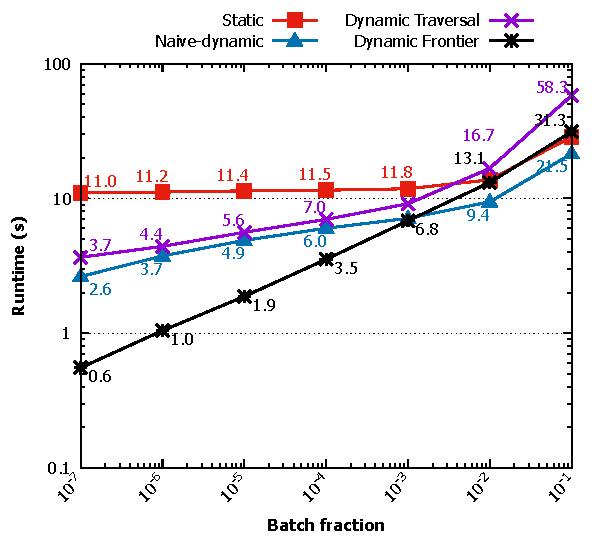
\includegraphics[width=0.38\linewidth]{out/insertions-runtime-mean.pdf}
  }
  \subfigure[Results on each graph]{
    \label{fig:insertions-runtime--all}
    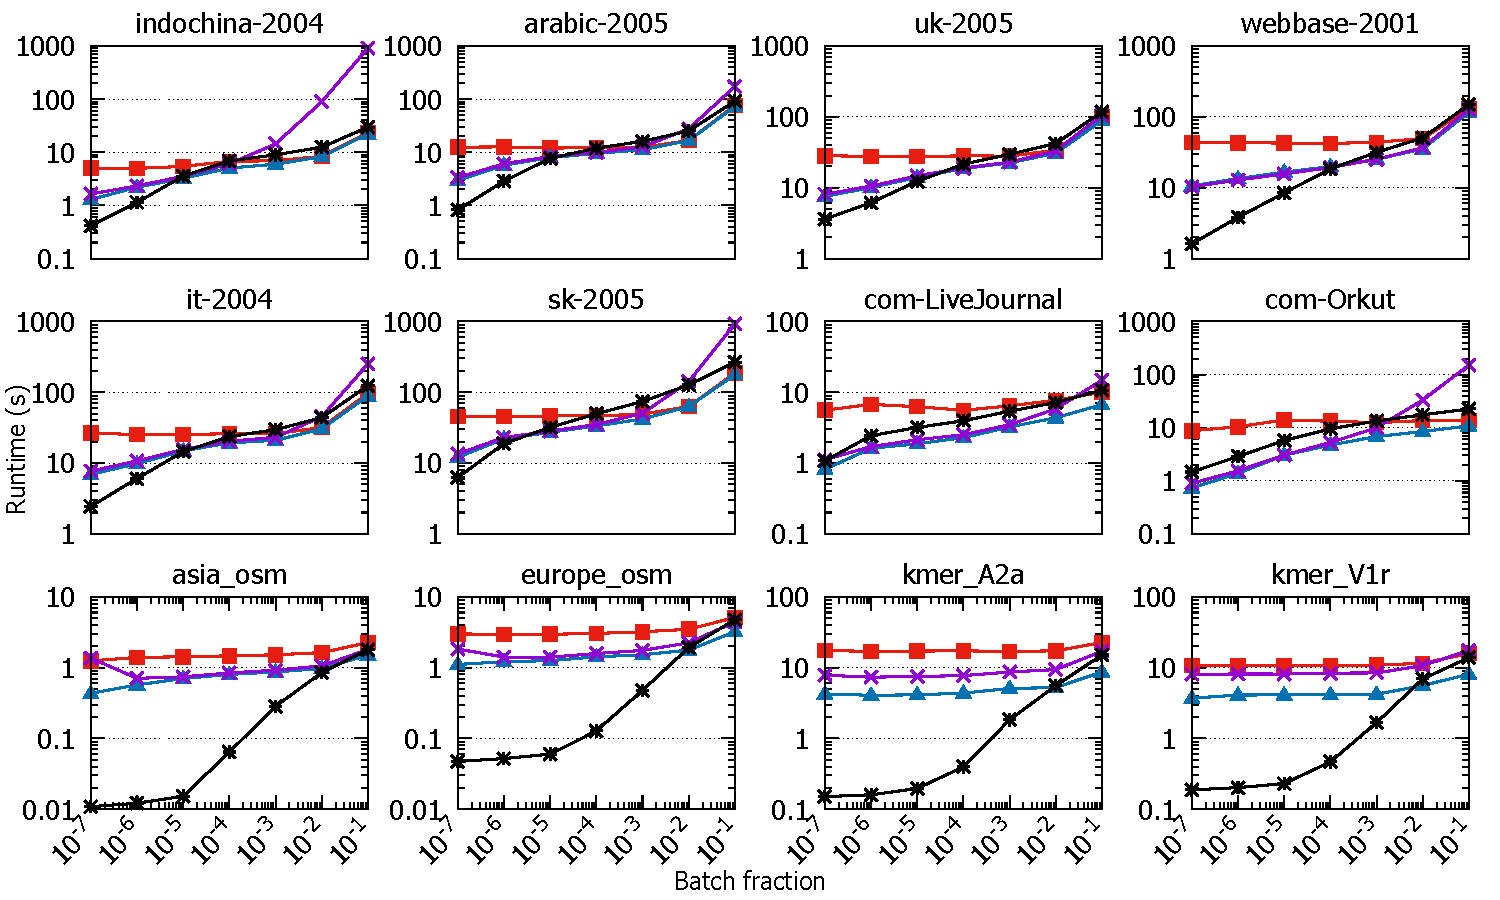
\includegraphics[width=0.58\linewidth]{out/insertions-runtime-all.pdf}
  } \\[-1ex]
  \caption{Runtime (logarithmic scale) for \textit{Static}, \textit{Naive-dynamic}, \textit{Dynamic Traversal}, and \textit{Dynamic Frontier} PageRank with batch updates exclusively comprising edge insertions, ranging from $10^{-7} |E|$ to $0.1 |E|$ in multiples of $10$ (logarithmic scale). The right figure details the runtime of each approach for individual graphs in the dataset, while the left figure displays overall runtimes --- using geometric mean for consistent scaling across graphs.}
  \label{fig:insertions-runtime}
\end{figure*}
